\section{Presentazione}
Tramite CSS è stato implementato un design fluido e scalabile, grazie all’utilizzo di misure sempre relative o in percentuale. Questo, oltre a migliorare l’accessibilità, permette una corretta visualizzazione delle pagine su tutti i formati di schermo, senza intaccare in alcun modo la navigazione tramite screen reader. Abbiamo quindi prodotto tre fogli di stile differenti, ciascuno per il target opportuno.

\subsection{Desktop}
Per una descrizione dettagliata dell'header consultare la sezione \ref{subsection:header}, per il contenuto la sezione \ref{subsection:contenuto}.\\
\begin{figure}[htbp]
	\begin{center}
		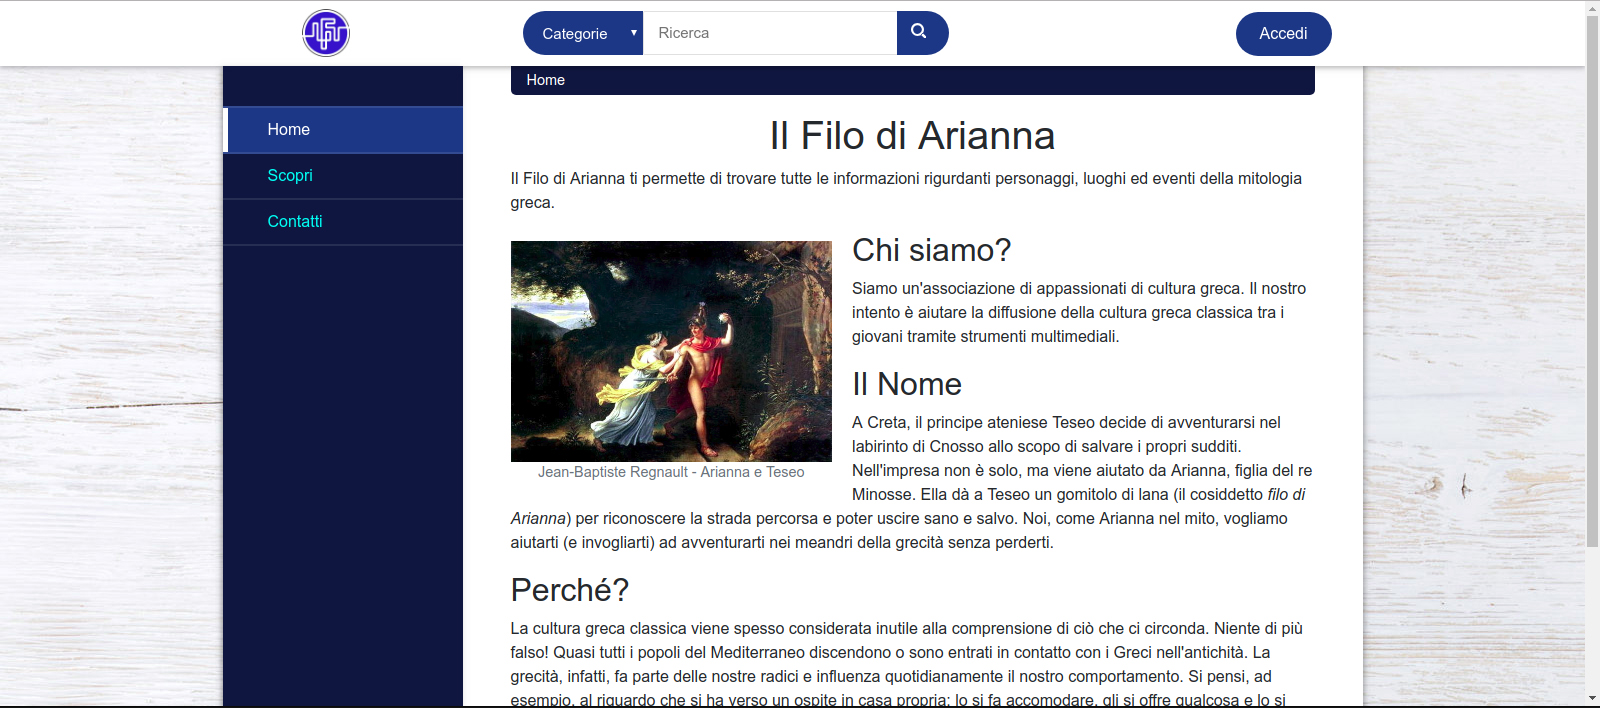
\includegraphics[width=13cm]{img/desktop.jpg}
		\caption{Visualizzazione Desktop}
	\end{center}
\end{figure}
\pagebreak
\subsection{Mobile}
Per quanto riguarda la visualizzazione per smartphone, il menu è nascosto al di fuori dell'area visibile del sito. Per farlo comparire basta premere il burger menu in alto a destra. Abbiamo scelto quel posizionamento perché il 49\% degli utenti usa lo smartphone ad una mano e il pollice come puntatore. Siccome la maggior parte di essi non è mancina, riusciranno a raggiungere più facilmente il pulsante. Per quanto riguarda l'altra percentuale di utenti, non avranno problemi al raggiungimento del pulsante perché usano lo smartphone a due mani. Per questi motivi il menu verrà visualizzato coprendo l'intera larghezza dello schermo con le voci al centro.\\
Per quanto riguarda la barra di ricerca, abbiamo deciso di rimuovere le categorie che comparivano a sinistra nella visualizzazione per Desktop perché andava ad occupare la maggior parte dello spazio di input e questo comportava una diminuzione della qualità di ricerca, come già menzionato nella sezione \ref{subsection:header}.
\begin{figure}[H]
	\begin{center}
		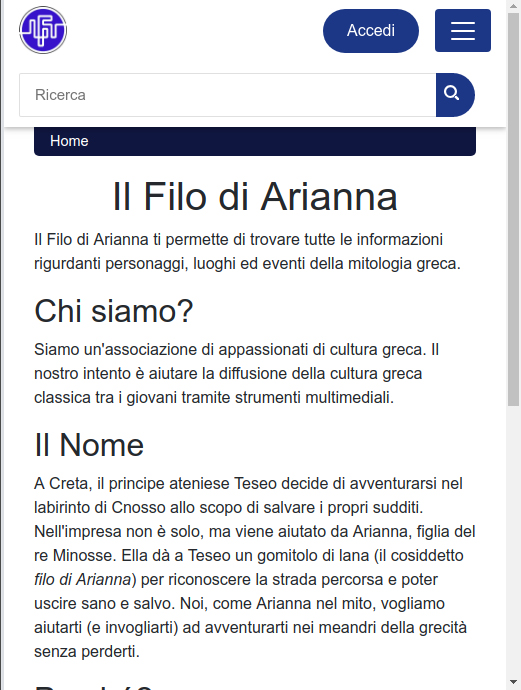
\includegraphics[width=9cm]{img/mobile.jpg}
		\caption{Visualizzazione Mobile}
	\end{center}
\end{figure}
\pagebreak
\subsection{Print}
Questo foglio di stile si applica automaticamente quanto un utente vuole
stampare la pagina. Come da usanza comune, sono stati tolti tutti gli elementi visivi non strettamente necessari al contenuto, quindi tutte le immagini
di background o di presentazione. Abbiamo rimosso anche il menu, la barra di ricerca, il footer e tutti i pulsanti, in quanto non ne abbiamo ritenuta fondamentale la visualizzazione su una pagina stampata. Inoltre abbiamo deciso di rendere le pagine in bianco e nero siccome il sito serve per fare ricerche, il contenuto è la cosa più importante, l'abbellimento grafico passa in secondo piano.
\begin{figure}[H]
	\begin{center}
		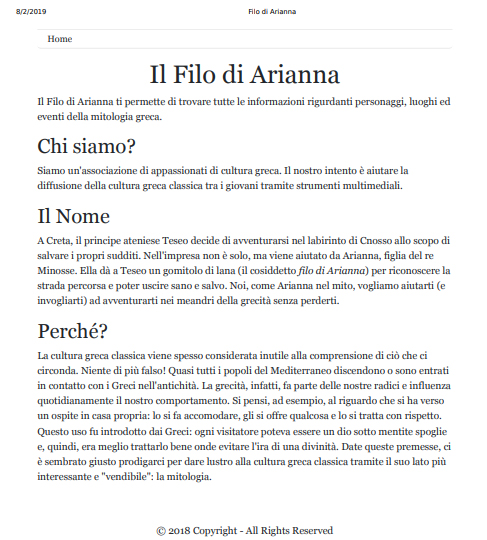
\includegraphics[width=9cm]{img/print.jpg}
		\caption{Visualizzazione di stampa}
	\end{center}
\end{figure}